\section{Mesh Router}

\begin{frame}{Software}
    \begin{itemize}
        \item OpenWRT mit
        \item Batman-Adv
        \item Fastd
        \item Nodewatcher
        \item Fastdstart
        \item .. weiteren kleineren Tools
        \item .. configs und scripten
    \end{itemize}
\end{frame}

\begin{frame}{von aussen}
    \begin{itemize}
        \item Client-Ports \& Infrastructure Funknetz:
            Wie ein großer Switch
        \item Batman-Ports \& Ad-Hoc Funknetz:
            Mesh-Netz
        \item WAN-Ports:
            VPN Netz
    \end{itemize}
    \center{
        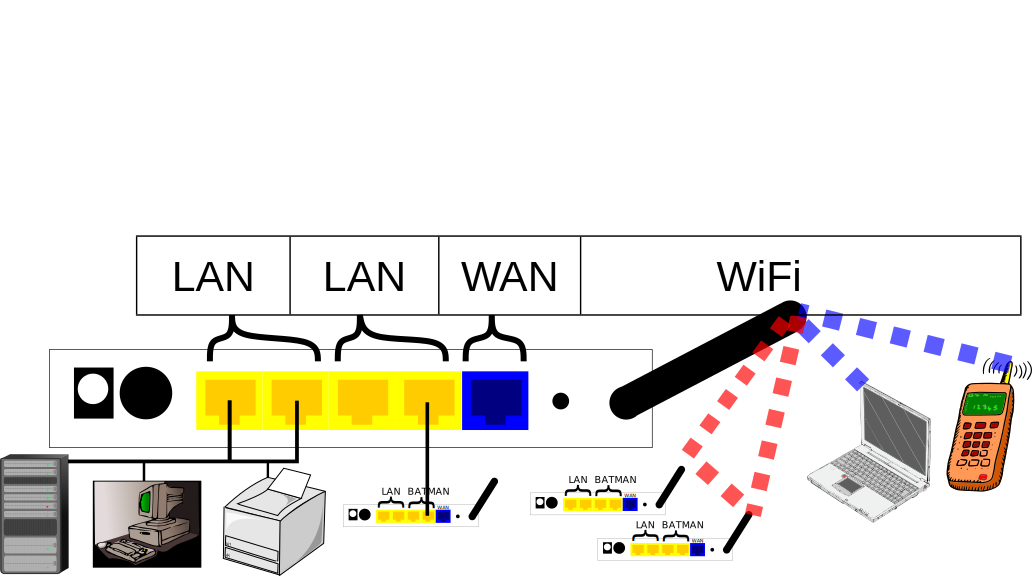
\includegraphics[width=0.75\textwidth]{img/svg/anschluesse.pdf}
    }
\end{frame}

\begin{frame}{von innen}
    \renewcommand{\arraystretch}{1.5}
    \begin{tabular}{|c|c|c|c|c|c|c|} \hline
         \multicolumn{7}{|c|}{Bridge} \\ \hline
         \multirow{2}{*}{Managed} &
         \multicolumn{4}{c|}{B.A.T.M.A.N} &
         \multicolumn{2}{c|}{\multirow{2}{*}{Client-VLan}} \\ \cline{2-5}
         & Ad-Hoc & VPN & \multicolumn{2}{c|}{Node-VLan} & \multicolumn{2}{c|}{} \\ \hline
         \multicolumn{2}{|c|}{Wifi} & WAN & LAN1 & LAN2 &
         LAN3 & LAN4 \\ \hline
    \end{tabular}

    \begin{itemize}
        \item Jeder Knoten ist wie ein großer Switch
    \end{itemize}
\end{frame}

